\chapter{Controlador de corriente} \chapterlabel{Informe/4-ControladorCorriente} \label{cap:ControladorCorriente}

En este capítulo se diseña y modela el circuito encargado de controlar la corriente que circula por el electroimán. Como se vio en el capítulo anterior, el sistema trabaja con corrientes elevadas por lo que se implementan estrategias de conmutación para reducir las pérdidas de energía. Para ello se utiliza una topología de puente H con cuatro MOSFET y un \textsl{driver} que los controla. Además, se detallan los criterios tenidos en cuenta al momento de  elegir  y dimensionar todos los componentes que intervienen para lograr el correcto funcionamiento del controlador de corriente. Por último, se obtiene su función transferencia  para ser utilizada en el diseño del compensador.

\section{Descripción general}\label{sec_descripcion-general}

Para mantener en suspensión a la pieza móvil es necesario regular la fuerza electromagnética generada por el electroimán. Esto se logra modificando la intensidad de la corriente que circula por su bobinado. Para ello, es necesario diseñar una fuente de alimentación que sea capaz de proveer la corriente requerida.

Para diseñar la fuente de alimentación se debe conocer el comportamiento eléctrico de la planta. Como se analizó en el capítulo \ref{cap:CaracterizacionElectroiman}, el electroimán puede ser modelado como una inductancia variable con una resistencia serie. Es decir, es un circuito RL serie cuya corriente ($I_L$) depende de la tensión aplicada ($V_L$). La expresión \ref{eq_corriente} muestra la relación entre estos parámetros.

\begin{equation} \label{eq_corriente}
\frac{I_L}{V_L}(s)=\frac{1}{sL(Y_g)\ +\ R_L}
\end{equation}

Al aplicar la transformada inversa de Laplace a la expresión  \ref{eq_corriente}, se puede obtener la respuesta temporal de la corriente ante un escalón de tensión de amplitud ``$v_L$'' en la entrada considerando condiciones iniciales $I_o$:

\begin{equation} \label{eq_corriente_temporal_cond_iniciales}
	i_L(t)=\frac{v_L}{R_L} + (I_o-\frac{v_L}{R_L})*e^{-\frac{t}{\tau}}
\end{equation}

En este caso particular $I_o=0$, por lo tanto la expresión para la corriente queda:

\begin{equation} \label{eq_corriente_temporal}
	i_L(t)=\frac{v_L}{R_L}*(1-e^{-\frac{R_L}{L(Y_g)}*t})
\end{equation}



En la expresión \ref{eq_corriente_temporal} se puede observar que la respuesta al escalón está compuesta por dos partes: un término con una exponencial negativa correspondiente al transitorio, y un término constante correspondiente al valor en régimen permanente $\frac{v_L}{R_L}$. El primero provoca que la corriente en el inductor crezca de manera amortiguada, hasta alcanzar el valor de régimen permanente luego de cierto tiempo. Este comportamiento se puede observar en la simulación realizada en la figura \ref{fig:img_respuesta_escalon}. En la parte superior de la figura se observa la tensión de entrada, y en la parte inferior la corriente del electroimán. Este análisis resulta de utilidad para conocer el comportamiento del electroimán y diseñar un controlador de corriente adecuado.


\begin{figure}[H]
	\centering
	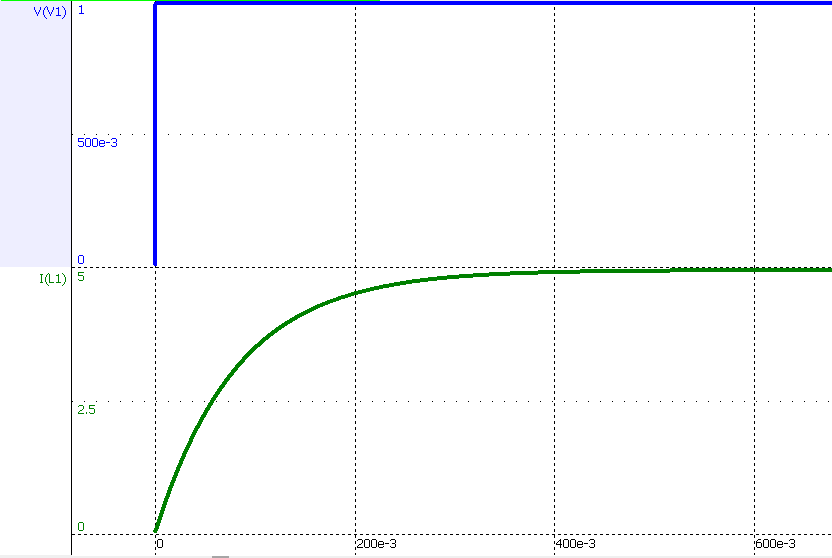
\includegraphics[scale=0.5]{corriente_escalon.png}
	\caption{Respuesta ante una entrada en escalón.}
	\label{fig:img_respuesta_escalon}
\end{figure}


\section{Diseño de la topología}


Se desea diseñar un sistema de control que modifique la alimentación del electroimán con el objetivo de que circule una corriente con un valor medio deseado por su bobinado.  Para ello, se propone implementar un sistema realimentado que compare la corriente que circula por el electroimán con una de referencia, que es la que se quiere que circule. En la figura \ref{fig:img_diagrama_bloques_basico} se muestra un diagrama en bloques simplificado del sistema.

\begin{figure}[H]
	\centering
	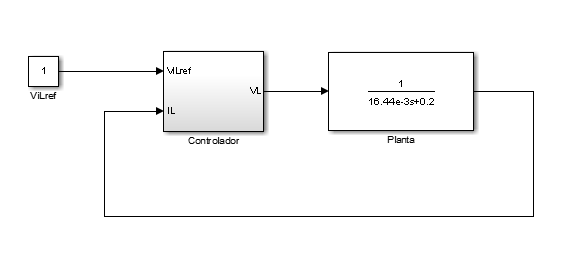
\includegraphics[scale=1]{Diagrama-en-bloques-basico.png}
	\caption{Diagrama en bloques básico del controlador de corriente.}
	\label{fig:img_diagrama_bloques_basico}
\end{figure}

De este diagrama surgen dos necesidades:
\begin{itemize}
	\item Diseñar un controlador que modifique la alimentación del electroimán según sus entradas.
	\item Medir la corriente que circula en el electroimán para poder utilizarla como entrada al controlador.
\end{itemize}

A continuación se analizan distintas alternativas para satisfacer estas necesidades.

\subsection{Control de corriente mediante transistor en modo lineal}

Como se analizó en la sección \ref{sec_descripcion-general}, el valor en régimen permanente de la corriente depende proporcionalmente de la tensión aplicada al electroimán. Por lo tanto, para mantener una corriente constante controlada se podría utilizar un transistor en modo lineal, es decir, como una fuente de corriente constante. 

Una posible implementación circuital se muestra en la figura \ref{fig:img_controlador-lineal}.

\begin{figure}[H]
	\centering
	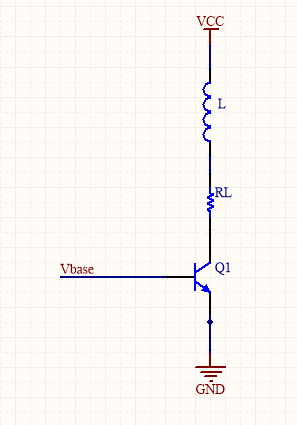
\includegraphics[scale=0.7]{controlador_lineal.png}
	\caption{Control de corriente mediante transistor en modo lineal.}
	\label{fig:img_controlador-lineal}
\end{figure}

En este modo de funcionamiento la tensión colector-emisor ($V_{CE}$) se controla de manera que la diferencia entre esta y la tensión de alimentación, circulando por la resistencia interna del electroimán, generen la corriente deseada. Es decir, en régimen permanente se obtiene:
 
 \begin{equation}
 	I_L=\frac{V_{CC}-V_{CE}}{R_L}
 \end{equation}
 
La desventaja de esto es que al circular una corriente constante, la caída de tensión sobre el inductor es prácticamente nula (solo lo correspondiente a la resistencia interna). Por lo tanto, la mayor parte de la potencia disipada cae sobre el transistor. Esta puede calcularse como: 

\begin{equation}
	P_{transistor} = I_L*V_{CE}
\end{equation}

Teniendo en cuenta que la tensión colector-emisor es la resta de la tensión de alimentación y la caida en la resistencia del electroimán:

\begin{equation}
	V_{CE}=V_{CC}-I_L*R_L
\end{equation}

Finalmente:

\begin{equation}
	P_{transistor}=V_{CC}*I_L-I_L^2*R_L
\end{equation}

Esta función llega a un máximo cuando $I_L=\frac{V_{CC}}{2*R_L}$


\begin{equation}\label{eq_pot_transistor_lineal_final}
	P_{transistor_{max}}=\frac{V_{CC}^2}{4*R_L}
\end{equation}

Teniendo en cuenta que la corriente maxima que se requiere es de aproximadamente 30 A se puede obtener que la minima tension de VCC requerida es:

\begin{equation}
	V_{CC}=I_L*R_L+V_{CE}=30 A * 0,2  = 5 V, VCE=0
\end{equation}

En el mercado las fuentes de tension capaces de entregar 30 A mas comunes en el mercado comienzan con valores minimos de 12 V. Si se reemplaza este valor en la ecuacion  \ref{eq_pot_transistor_lineal_final} se obtiene un valor minimo de 180 Watt, esto elevaria demasiado la temperatura del transistor, haciendo que sea necesario el agregado de un gran disipador de calor y pone en riesgo la vida útil de los componentes.
  
En la ecuación \ref{eq_pot_transistor_lineal_fina} se puede ver que para valores de tension normalmente utilizados $(5\:V,10\:V,15\:V)$ la potencia disipada por el transistor varía entre $30\:W$ hasta $280\:W$. Esto eleva demasiado la temperatura del transistor, haciendo que sea necesario el agregado de un gran disipador de calor y pone en riesgo la vida útil de los componentes.

Aunque aún no se define con qué tensión se alimentará el sistema, se puede probar con valores utilizados comunmente para obtener una aproximación de la potencia disipada por el transistor. Por ejemplo, para valores de tensión de alimentación $(5\:V,10\:V,15\:V)$ el valor de potencia que se obtiene varía entre $30\:W$ hasta $280\:W$. Esto eleva demasiado la temperatura del transistor, haciendo que sea necesario el agregado de un gran disipador de calor y pone en riesgo la vida útil de los componentes.

\colorbox{red}{HACER UN MEJOR ENGANCHE}

\subsection{Control de corriente mediante conmutación}

Como se analizó en la sección anterior, al trabajar con corrientes elevadas, no es eficiente utilizar un transistor que trabaje en su zona lineal puesto que el consumo de energía es elevado. Se propone entonces utilizar una fuente conmutada.

%\noindent Para lograr una corriente continua en el electroimán mediante una fuente conmutada se debe alternar la polaridad de la tensión aplicada en sus bornes. De esta forma, se aprovecha el transitorio mostrado en la figura \ref{fig:img_respuesta_escalon} para hacer crecer la corriente hasta llegar a un cierto valor (denominado límite superior), y luego se conmuta la polaridad de la alimentación para que decrezca. Nuevamente, al llegar a un cierto valor (denominado límite inferior), se vuelve a conmutar. Este proceso se repite, y se logra que la corriente oscile en torno al valor medio entre los dos límites, que es el valor de corriente continua deseado. 

Al aplicar tensión en los bornes del electroimán, la magnitud de la corriente aumentará en forma exponencial. Si se desea que la corriente que circule por su bobinado sea aproximadamente continua, es necesario alternar la polaridad de la tensión aplicada ($\pm V_L$) de forma que la corriente oscile en torno al valor medio deseado ($<I_L>$) como se observa en la figura \ref{fig:img_corriente_exponencial}.

\begin{figure}[H]
	\centering
	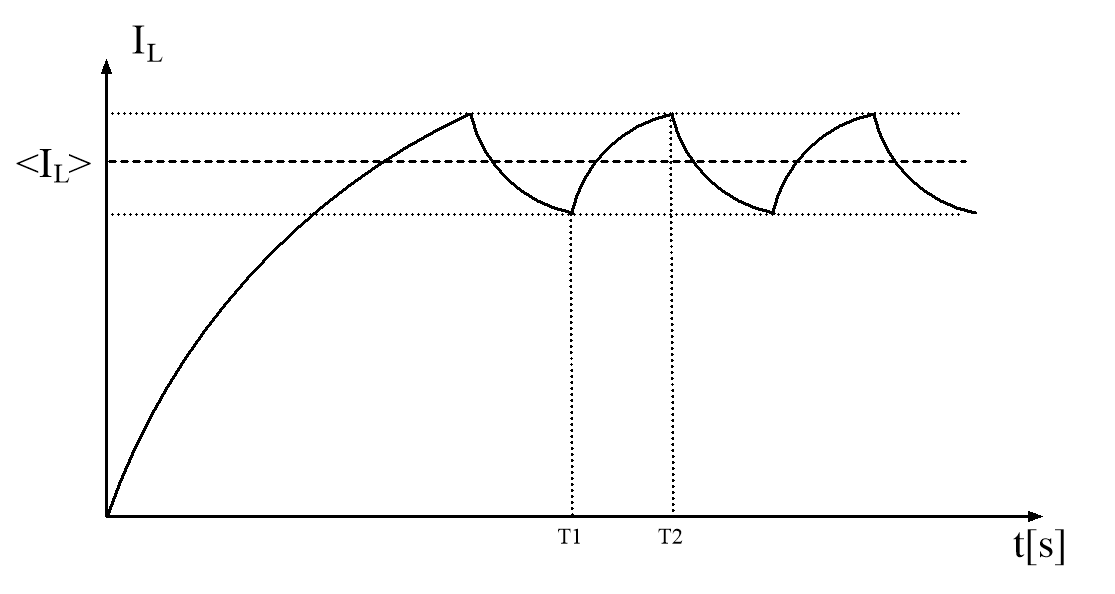
\includegraphics[scale=0.5]{Forma-de-onda-corriente-exponencial.png}
	\caption{Forma de onda de corriente y tensión en el electroimán.}
	\label{fig:img_corriente_exponencial}
\end{figure}

%En la figura \ref{fig:img_corriente_exponencial} se puede ver que la corriente crece y decrece en forma exponencial dentro de cada ciclo de conmutación. Sin embargo, si se elige un intervalo de tiempo de la conmutación pequeño comparado con la constante de tiempo de la planta, el incremento de corriente será pequeño y puede ser aproximado como una rampa. Por lo tanto, se obtiene una corriente continua con un ripple superpuesto de forma triangular, como la que se muestra en la figura \label{fig:img_corriente_lineal}.

%\begin{figure}[H]
%	\centering
%	\includegraphics[scale=0.5]{forma-de-onda-corriente-lineal.png}
%	\caption{Forma de onda de corriente al disminuir el período de conmutación.}
%	\label{fig:img_corriente_lineal}
%\end{figure}

Por lo tanto, es necesario diseñar un circuito que permita alternar la polaridad de la tensión aplicada al electroimán y controlar el valor medio de su corriente. Entre las distintas topologías de fuentes conmutadas que se utilizan comúnmente, una que tiene la capacidad de alimentar su carga en ambos sentidos es la topología de puente completo con cuatro llaves que se muestra en la figura \ref{fig:img_topologia_simplificada}.

\begin{figure}[H]
	\centering
	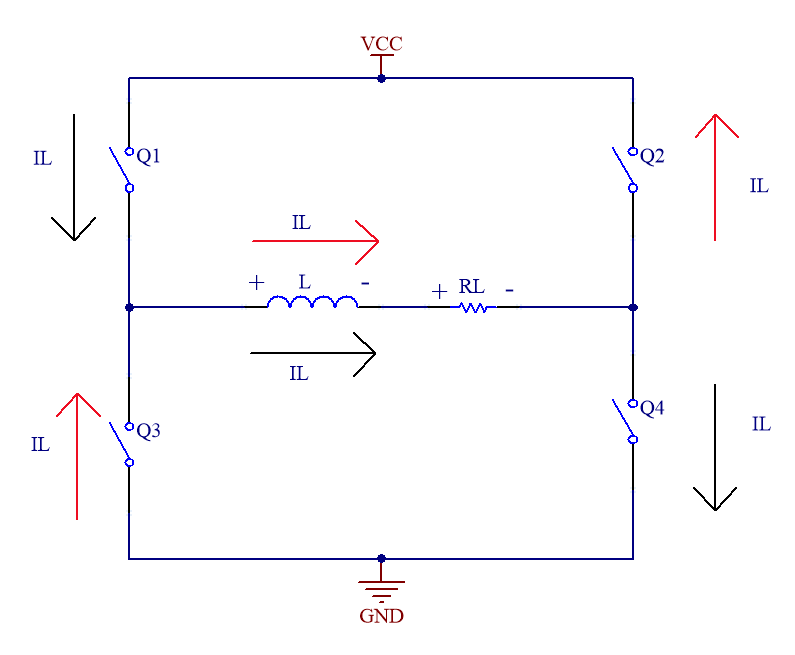
\includegraphics[scale=0.5]{puente_con_llaves.png}
	\caption{Topología simplificada.}
	\label{fig:img_topologia_simplificada}
\end{figure} 


El electroimán se conecta entre los puntos medios de cada par de llaves. Cada una de ellas puede ser controlada de manera independiente mediante señales eléctricas. A través de una combinación correcta de las mismas se puede controlar la polaridad de la alimentación y el sentido de circulación de la corriente, según se desee. Para esta aplicación en particular, la fuerza magnética es siempre en el mismo sentido, independientemente del sentido en que circule la corriente. Por lo tanto, se adopta como sentido de circulación positivo de izquierda a derecha como lo indican las flechas en la figura \ref{fig:img_topologia_simplificada}.

Para poder obtener una forma de onda de corriente como la que se muestra en la figura \ref{fig:img_corriente_exponencial}, comenzando desde corriente nula, se debe controlar el estado de las llaves de la siguiente manera:

\begin{itemize}
	\item En principio se cierran las llaves $Q_1$ y $Q_4$ a la vez, generando un circuito entre $V_{cc}$, el electroimán y GND como indican las flechas negras en la figura \ref{fig:img_topologia_simplificada}. De esta forma, la corriente comienza a crecer con forma de exponencial negativa. 
	\item Al llegar al límite superior ($I_{MAX}$), el controlador conmuta el estado de las llaves, de manera que $Q_1$ y $Q_4$ dejan de conducir, y comienzan a hacerlo $Q_2$ y $Q_3$. De esta manera, la corriente seguirá circulando en el mismo sentido como indican las flechas rojas, pero ahora la diferencia de potencial en los bornes del electroimán se opone al paso de la corriente, por lo que su magnitud comienza a decrecer.
	\item Una vez alcanzado el límite inferior ($I_{MIN}$), el controlador vuelve a conmutar el estado de las llaves para que la corriente tenga pendiente positiva.
\end{itemize}

Este ciclo se repite en régimen permanente para obtener la corriente deseada. Si se elige un tiempo de conmutación pequeño comparado a la constante de tiempo de la planta, la fuerza magnética producida por esta corriente oscilante podrá ser filtrada, quedando únicamente su valor medio. Es decir, no habrá variaciones significativas en la fuerza ejercida.

Es importante tener en cuenta que sólo dos llaves pueden encenderse a la vez, y esto debe realizarse de manera diagonal. Es decir, en la figura \ref{fig:img_topologia_simplificada}, $Q_1$ y $Q_4$ pueden estar encendidos, mientras que $Q_3$ y $Q_2$ están apagados, y viceversa. Esto es debido a que se podría generar un cortocircuito entre la fuente de alimentación y GND, produciendo una circulación de corriente elevada que podría dañar el sistema y la fuente de alimentación. Se debe tener en cuenta esta restricción al momento de diseñar el circuito encargado de controlar estas llaves.

Por otro lado, al considerar que el tiempo de conmutación es pequeño comparado a la constante de tiempo de la planta, la forma de onda de la corriente en régimen permanente será triangular puesto que no llegará a tomar forma exponencial. Además, como la tensión aplicada a los bornes del electroimán en cada semiciclo de conmutación es igual en magnitud y el circuito de carga y descarga del electroimán es el mismo, la onda triangular tendrá pendientes simétricas. La forma de onda resultante se puede observar en rojo en la figura \ref{fig:img_corriente_triangular}.

\begin{figure}[H]
	\centering
	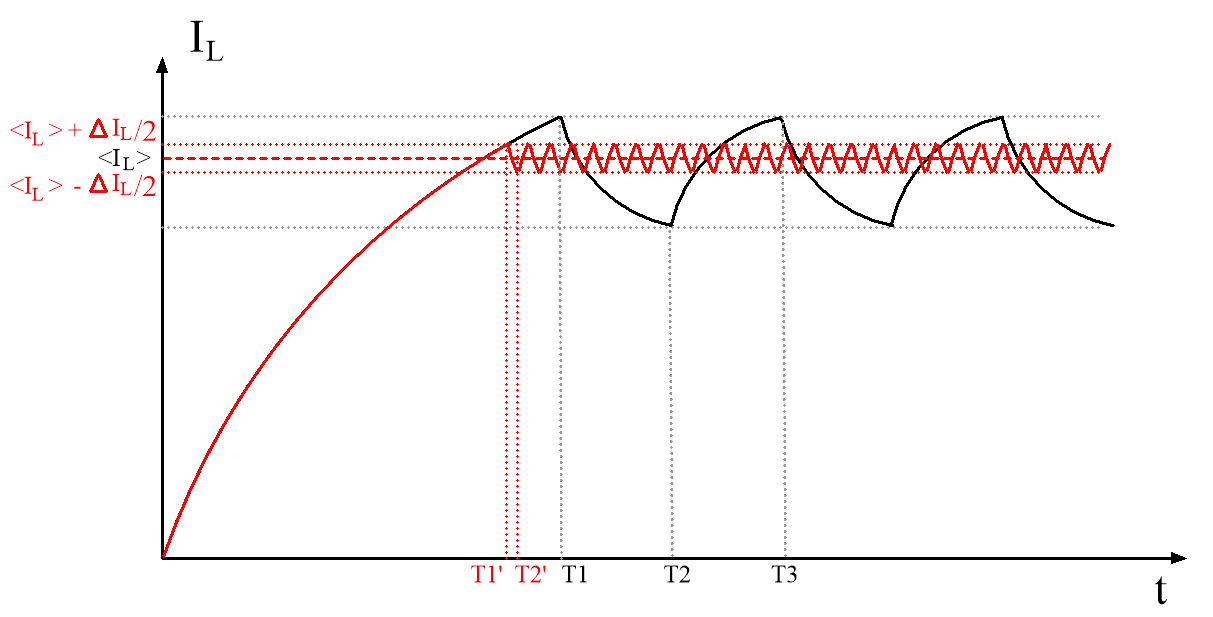
\includegraphics[scale=0.5]{Forma-de-onda-corriente-lineal.png}
	\caption{Forma de onda de corriente triangular}
	\label{fig:img_corriente_triangular}
\end{figure} 

Como se mencionó previamente, para obtener el valor medio de corriente deseado es necesario controlar el tiempo que se le aplica cierta polaridad de tensión al electroimán. Para ello, se debe actuar sobre las llaves en función de si se desea que la corriente aumente o disminuya.

Una manera de implementar la lógica de control es mediante un controlador de lazo cerrado del tipo ON-OFF. En la figura \ref{fig:img_diag-en-bloques-comparador-sin-hist} se muestra su diagrama en bloques. Este controlador realiza una resta entre la corriente de referencia y la corriente que está circulando por el electroimán, para obtener un valor llamado corriente de error (Ie). De esta forma, si la corriente medida es menor a la de referencia, la polaridad de la tensión aplicada en los bornes del electroimán, será positiva para lograr que su corriente crezca e iguale a la de referencia. En cambio, si resulta mayor, la alimentación será negativa para disminuir la corriente.


\begin{figure}[H]
	\centering
	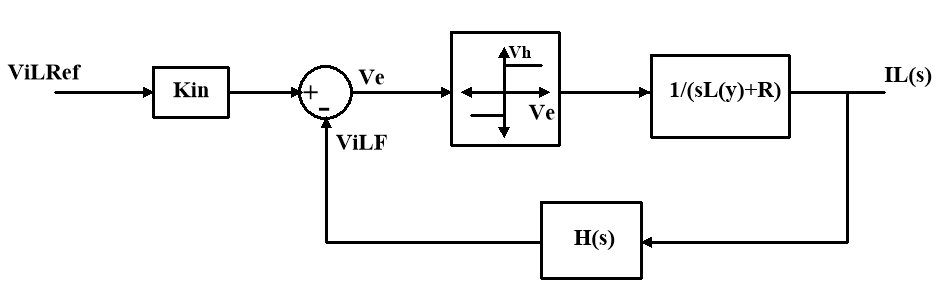
\includegraphics[width=\textwidth]{Diagrama-en-bloques-comparador-sin-hist.png}
	\caption{Diagrama en bloques simplificado del controlador de corriente.}
	\label{fig:img_diag-en-bloques-comparador-sin-hist}
\end{figure}

Al analizar el diagrama en bloques planteado en la figura \ref{fig:img_diag-en-bloques-comparador-sin-hist} es posible notar que, una vez que la corriente del electroimán (IL(s)) supere infinitesimalmente a la referencia, se produce una conmutación en la polaridad de tensión aplicada al electroimán. Lo mismo sucede cuando es infinitesimalmente menor. El inconveniente que esto presenta es que se producirían conmutaciones extremadamente rápidas en torno al valor medio, por lo que sería necesario tener alta velocidad en conmutación. Por lo tanto, para reducir la frecuencia de esas oscilaciones, resulta conveniente agregar histéresis al controlador, de la manera que se muestra en la figura \ref{fig:img_diag-en-bloques}.

\begin{figure}[H]
	\centering
	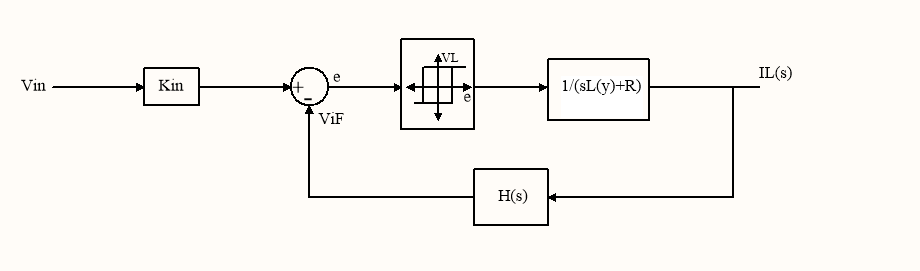
\includegraphics[width=\textwidth]{Diagrama-en-bloques.png}
	\caption{Diagrama en bloques del controlador de corriente con un comparador con histéresis.}
	\label{fig:img_diag-en-bloques}
\end{figure}

Este bloque permite definir un margen de corriente $\Delta I_L$ de forma tal que, si la corriente que circula por el electroimán supera a la de referencia, no se producirá un cambio de polaridad en la tensión aplicada hasta que la supere por $\frac{\Delta I_L}{2}$. Análogamente, cuando comienza a decrecer, seguirá haciéndolo hasta que sea menor a la corriente de referencia menos $\frac{\Delta I_L}{2}$.

PONER IMAGEN EXPLICANDO HISTERESIS


Debido a que lo único que cambia es la polaridad de la tensión con la que se excita al electroimán, la constante de tiempo del circuito no cambia. Esto da como resultado  que la corriente oscile sobre un valor medio con igual tiempo de crecimiento como de decrecimiento. Esta oscilación también es conocida como ripple. Su ancho es fijo y está determinado por el ancho de histéresis que con el que se diseñe el controlador. 

Para elegir un ancho de histéresis adecuado se debe tener en cuenta que, al analizar la forma de la corriente en la figura \ref{fig:img_corriente_triangular} se deduce que a mayor $\Delta I_L$, se tiene una menor frecuencia de oscilación. 

Como se mencionó, se desea controlar la fuerza ejercida a partir del valor medio de la corriente. Por lo tanto, las variaciones en torno a dicho valor medio no deben generar variaciones significativas en la fuerza magnética. Por ello, se debe elegir un ancho de histéresis tal que la frecuencia de conmutación resultante sea al menos 100 veces mayor que la frecuencia del polo de la planta obtenida en \ref{eq_transferencia_planta_m}. Este se ubica en $70\:r/s$, lo que resulta en que se debe conmutar a una frecuencia de $\omega_{sw}>=7000\:r/s$, y expresada en Hz resulta $F_{sw}>=1\:kHz$.

\colorbox{red}{Esto conviene calcularlo acá o dejarlo planteado y calcular mas adelante?}

Por lo tanto, como la frecuencia mínima es $F_{sw}$, y considerando que el tiempo en que crece la corriente es igual al que decrece, se obtiene que el tiempo máximo que puede tener la sección creciente de la corriente es igual a $t_{max}=500\:us$. 

A partir de la expresión \ref{eq_corriente_temporal_cond_iniciales} se puede obtener el valor máximo de ripple cuando $t=t_{max}$, considerando que la corriente inicial es $I_{min}$ y que la corriente final es $I_{min}+\Delta I_L$

\begin{equation} \label{eq_delta_i}
	I_{min}+\Delta I_{L_{max}}=\frac{v_L}{R_L}+(I_{min}-\frac{v_L}{R_L})*e^{-\frac{t_{max}}{\tau}}
\end{equation}

De la ecuación \ref{eq_delta_i} se puede despejar el valor máximo que puede tener $\Delta I_L$. 

\begin{equation} \label{eq_delta_i_2}
	\Delta I_{L_{max}}=6.06*10^{-3}*(\frac{v_L}{R_L}-I_{min})
\end{equation}

\colorbox{red}{HAY QUE DEFINIR VL ANTES DE ESTO} O DEJAMOS ESTA EXPRESIÓN Y DESPUÉS CUANDO CALCULAMOS VL CALCULAMOS EL DELTA I

\colorbox{red}{Para los calculos usé Vl=24V}


Sabiendo que el controlador de corriente tendrá una corriente media variable entre 0 y 30 A, se debe satisfacer la expresión \ref{eq_delta_i_2} para cualquier $I_{min}$ dentro de ese rango. Por lo tanto se plantean dos casos: $I_{min}=0$ e $I_{min}=30$. Para el primer caso se llega a que $\Delta I_{L_{max}}=727\:mA$ y en el segundo $\Delta I_{L_{max}}=500\:mA$. Por lo tanto se elige un ancho de histéresis de $500\:mA$ ya que cumple las dos condiciones.



\colorbox{red}{esto no se si va}
Como se mencionó, la forma de onda tendrá un ripple en torno a un valor medio. La elección del ancho de este ripple determinará la velocidad de respuesta que el comprador pueda tener. Esto quiere decir que el error ($I_{e}$(cambiar desp a Ie en la figura)) aumentará hasta cierto valor definido para luego ser corregido. Si $I_{e}$ alcanza un valor demasiado grande la pieza que se desea mantener levitando caerá debido a que el sistema no conmutó lo suficientemente rápido, caso contrario, si la conmutación es muy rápida traerá los problemas ya mencionados anteriormente.

Sensado de corriente

Como se puede ver en el diagrama en bloques anterior, para poder realizar la comparación es necesario realimentar la corriente del electroimán para que el comprador pueda actuar en función al error ($I_{e}$).

Para hacer esto se debe utilizar un sensor que permita una medición de corriente mayor a 31 amperes y con un error máximo tolerable tal que permita actuar al comparador y no afecte al sistema. Además lo de la conmutación q dijo el gusti…

Los sensores de corriente trabajan en transresistencia, por lo tanto, se agrega el bloque H en el lazo de realimentación figura \ref{fig:img_diag-en-bloques-conH-y-Kin}. Ahora $V_{iL}=i_{L}*rm$. De esta forma ahora se está trabajando con tensiones por lo tanto la corriente de referencia se afecta por el bloque $K_{in}$ para obtener su equivalente en tensión. El bloque resultante es el siguiente:

\begin{figure}[H]
	\centering
	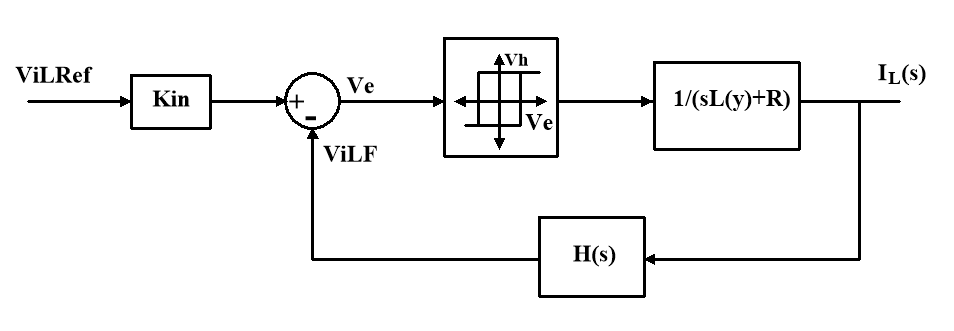
\includegraphics[width=\textwidth]{Diagrama-en-bloques-conH-y-Kin.png}
	\caption{Diagrama en bloques del controlador de corriente completo.}
	\label{fig:img_diag-en-bloques-conH-y-Kin}
\end{figure}

Se puede expresar al error que introduce el sensor de efecto hall como $V_{errSensor}$. Entonces la expresion de error $V_{e}$ resulta: 

\begin{equation}\label{eq_error_ve}
	V_{e}= K_{in}*I_{ref}-H*iL\pm V_{errSensor}=\triangle I \pm V_{errSensor}
\end{equation}

	

De esta forma, tomando el  caso extremo $K_{in}*I_{ref}=H*i_{L}$ el error obtenido $V_{e}=\pm V_{errSensor}$.
Es decir que el error es el propio error del sensor. Si se toma un ancho de histéresis mucho mayor al error máximo introducido por el sensor, este error no afectaría al sistema ya que seria despreciable a comparación del valor que deltaI debería alcanzar para que el comparador cambie de estado.

El error que introduce el sensor de efecto hall $V_{errSensor}$ debe ser mucho menor al ancho de histéresis del comparador.


\section{Elección de tensión de alimentación}

Para comenzar el diseño circuital es importante determinar cómo será la alimentación del controlador de corriente. Para definirla se tendrá en cuenta la velocidad de respuesta de la planta que está determinada por el polo dominante. 

Al analizar la forma de corriente de la FIGURA 3.6, se observan tres secciones de tiempo diferenciadas. La que es de interés para este análisis es desde que el equipo se enciende(t0) hasta cuando actúa el comparador(t1). Al encender el equipo el electroimán puede encontrarse en cualquier punto. Si este se encuentra muy alejado tal que la corriente necesaria para mantenerlo sea mayor a la corriente máxima(Imax) el objeto se caerá. Otro caso es que el objeto esté a una distancia Y que el sistema deberá mantener. Para hacerlo el sistema iniciará con corriente nula hasta alcanzar el valor necesario para mantener al objeto levitando. Como el polo dominante ya está definido por el circuito RL del electroimán, la velocidad con que el sistema pueda alcanzar un valor de corriente elevado está determinado por el valor de la fuente de alimentación.

La expresión teórica de la corriente es: 

\begin{equation}
	I_L(t)=\frac{V}{R_L} + (I_o-\frac{V}{R_L})*e^{-\frac{t}{\tau}}
\end{equation}

Donde:
\begin{itemize}
	\item V es la tensión de alimentación, que puede tomar valores $+V_{cc}$ y $-V_{cc}$.
	\item $I_o$ es la corriente inicial en cada tramo de la imagen.
	\item $\tau$ es la constante de tiempo del electroimán.
\end{itemize}

Para encontrar la expresion del tiempo que tarda la corriente en alcanzar el valor maximo de corriente imax se reemplaza I0=0 y se obtiene T1. Esto da:

\begin{equation}\label{eq_tiempo_de_subida}
		T1=-\tau*ln(\frac{V_{cc}-R*I_{max}}{V_{cc}})
\end{equation}

Suponiendo que el electroimán se enciende en a una distancia de trabajo $Y=3 mm$, la corriente que se requiere es I=(buscar). Es necesario que el tiempo de subida de corriente T1 sea mucho menor al tiempo en que la carga llegue a la distancia máxima que el sistema soporta $Y=5mm$ aprox (que corresponde a imax). Es decir que el objeto cae libremente un delta $\Delta Y= 2mm $. Utilizando la ecuación que calcula el tiempo (T) que tarda en desplazarse un objeto en caída libre una altura $\Delta Y$:


\begin{equation}
	T=\sqrt{\frac{2*\Delta Y}{g}}
\end{equation}

Considerando $\Delta Y=2\:mm$, se llega a que $T=20,2 mSeg 17.5\:ms$. Por lo tanto se desea que $T1<T$.

Finalmente se obtiene: $Vcc=20.9\:V$.

----------------------------------------------------------------
SEPARADOR
------------------------------------------------

Otra 
Corriente para 4mm 30 KG = 16.3 A

Corriente para 4mm 1kG= 2.9 A

Hay que subir hasta 16.4 para que no se caiga el electroiman antes de que se nos valla a 5mm es decir delta Y=1mm.

T de caida libre(1mm)= 14,27 mSeg

Vcc necesario para que la corriente suba desde 2,9 a 16,3 en 14,27 mSeg es 16,77 V. 
si ponemos 24 va a tardar menos. Todo esto es sin considerar la fuerza magnética presente al inicio ni que esta aumenta a medida que la corriente sube. Es decir un caso que no va a existir que es el peor de todos lo cumplimos XD

----------------------------------------------------------------
SEPARADOR
------------------------------------------------
\section{2Elección de tensión de alimentación}
\colorbox{red}{Esto no iria acá, pero lo pongo para que ya quede y después lo movemos}

Para comenzar el diseño circuital es importante determinar cómo será la alimentación del controlador de corriente. Para definirla se tendrá en cuenta la velocidad de respuesta de la planta.... y nose que mas

analizando la forma de corriente de la FIGURA 3.6, se observan tres secciones de tiempo diferenciadas: desde t= 0 hasta t1, desde t1 hasta t2,  y desde t2 hasta t3. \colorbox{red}{marcar en la imagen}

Se puede encontrar la expresión teórica de la corriente para cada uno de esos instantes de tiempo... Se utiliza la formula:

\begin{equation}
	I_L(t)=\frac{V}{R_L} + (I_o-\frac{V}{R_L})*e^{-\frac{t}{\tau}}
\end{equation} 

Donde:
\begin{itemize}
	\item V es la tensión de alimentación, que puede tomar valores $+V_{cc}$ y $-V_{cc}$.
	\item $I_o$ es la corriente inicial en cada tramo de la imagen.
	\item $\tau$ es la constante de tiempo del electroimán.
\end{itemize}

Como el ancho del ripple de corriente es fijo y conocido (SE SUPONE QUE YA LO DEFINIMOS???) nos interesa NOSE QUE NOS INTERESA...



Para encontrar expresiones del tiempo que tarda en realizarse cada tramo, se reemplaza $I_o$ por la correspondiente y se obtiene el tiempo que tarda en llegar a la corriente final...


\begin{equation}
		T1=-\tau*ln(\frac{V_{cc}-R*I_{max}}{V_{cc}})
\end{equation}


\colorbox{red}{Con esta} podemos ver cuánto tardaríamos de pasar de corriente 0 a corriente máxima, y podemos decir que queremos tardar menos de cierto tiempo.


Por ejemplo usando la ecuación que calcula el tiempo (T) que tarda en desplazarse un objeto en caida libre una altura $\Delta Y$:

\begin{equation}
	T=\sqrt{\frac{2*\Delta Y}{g}}
\end{equation}

Considerando $\Delta Y=1.5\:mm$, se llega a que $T=17.5\:ms$. Por lo tanto se desea que $T1<T$.
finalmente se obtiene: $Vcc=20.9\:V$.



----------------------------------------------------------------
SEPARADOR
------------------------------------------------


Otra forma de calcular la tensión de alimentación que se necesita sería considerando que se desea que los tiempos de crecimiento sean lo mas parecidos posible a los de decrecimiento. Esta diferencia se hace mas pronunciada a medida que aumenta el valor medio de la corriente del electroimán.

\begin{equation}
	T2-T1=-\tau*ln(\frac{I_{min}+\frac{V_{cc}}{R}}{I_{max}+\frac{V_{cc}}{R}})
\end{equation}

\begin{equation}
	T3-T2=-\tau*ln(\frac{I_{max}-\frac{V_{cc}}{R}}{I_{min}-\frac{V_{cc}}{R}})
\end{equation}


Podemos poner todo en función de $I_{min}$ utilizando la relación $I_{max}=I_{min}+\delta I_L$

\begin{equation}
	T2-T1=-\tau*ln(\frac{1}{1+\frac{\Delta I_L}{I_{min}+\frac{V_{cc}}{R}}})
\end{equation}

\begin{equation}
	T3-T2=-\tau*ln(1+\frac{\Delta I_L}{I_{min}-\frac{V_{cc}}{R}})
\end{equation}


Podemos decir que queremos que estos tiempos sean lo mas parecidos posible, dentro de todo el rango de trabajo de la corriente. Para ello consideramos que T3 no debe hacerse mucho mayor que T2 en el caso de que la corriente sea la máxima (30 A). Por elegir un número, considero que T3 debe ser menor a $2*T2$ \colorbox{red}{tuve que elegir que sea menor al doble así me quedaba bien el} cruce de las figuras.  planteamos una inecuación y la resolvemos con un grafico:

\begin{figure}[H]
	\centering
	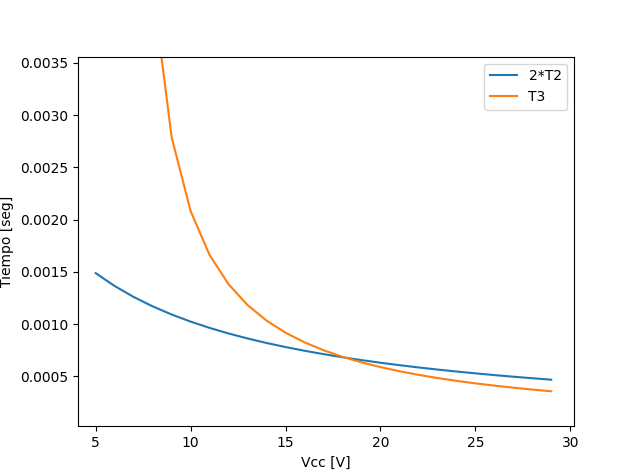
\includegraphics[width=\textwidth]{tiempos_conmutacion_vs_fuente.png}
	\caption{Tiempos de conmutación vs tensión de alimentación.}
	\label{fig:img_tiempos_conmutacion}
\end{figure}

El punto en que ambas figuras se cruzan es con $Vcc=18\:V$, por lo tanto se eligen una tensión de alimentación de $24\:V$.


\section{Diseño del circuito}

Se realizará el diseño circuital de cada bloque planteado en la figura \ref{fig:img_diag-en-bloques-conH-y-Kin}.

\subsection{Diseño de puente H}

capaz acá entraría lo del calculo de la fuente de alimentación

Para el diseño del puente H se deben definir qué componente electrónico cumplirá la función de actuaar como llave, proporcionar su circuitería de control, hip, bootstrap, todo eso

Como se mencionó previamente, se utiliza una topología de puente completo con 4 llaves para alimentar el electroimán. Para realizar una implementación circuital de ella, es necesario elegir qué componente electrónico cumplirá el rol de llave. Además se debe diseñar la circuitería necesaria para el correcto funcionamiento de las llaves.


\subsection{realimentacion}
capaz acá habría que poner lo del sensor de efecto hall?? y lo del operacional que hace la resta de vbias
asd


\subsection{etapa de entrada y restador}


Se plantea la etapa de entrada que consiste en la ganancia $K_{in}$ y el restador con la señal realimentada. Como se mencióno MAS ARRIBA, la etapa de entrada tiene una ganancia. Esta debe ser implementada con un circuito de operacionales.

La salida de esta etapa, al igual que la tensión de salida del sensor de efecto Hall, se polarizan en un punto de operación de $2.5\:V$ Para lograrlo se utiliza un circuito como el que se muestra en la figura \ref{fig:img_etapa-de-entrada}.


\begin{figure}[H]
	\centering
	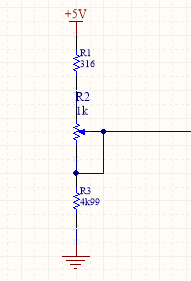
\includegraphics[scale=1]{Etapa-de-entrada.png}
	\caption{Etapa de entrada.}
	\label{fig:img_etapa-de-entrada}
\end{figure}
\colorbox{red}{Capaz sería mejor poner las imagenes directamente de Altium}

Las ecuaciones de diseño para este circuito son: ......


\subsection{comparador con histeresis}

Para la implementación del comparador con histéresis se utiliza un amplificador operacional realimentado positivamente. Se eligió que la corriente de salida del electroimán tenga un ripple de $500\:mA$. Por lo tanto, al afectar este valor por la transconductancia del sensor de efecto Hall, se obtiene un ancho de histéresis de $26.665\:mV$, alrededor de un punto de operación de $2.5\:V$. El circuito implementado se muestra en la figura \ref{fig:img_comp-con-hist}.

\begin{figure}[H]
	\centering
	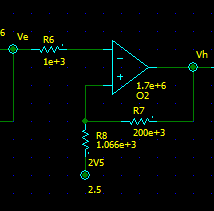
\includegraphics[scale=1]{Comparador-con-histeresis.png}
	\caption{Comparador con histéresis.}
	\label{fig:img_comp-con-hist}
\end{figure}

\subsection{conmutación auxiliar}
qqqwqw
\subsection{set-point de 2.6V}
 